\section{Un peu de contexte}

% \subsection{Les acteurs}
% \paragraph{}
% Ces travaux sont menés conjointement par le \gls{lifo} et la société \gls{ennov}.
% \gls{ennov} est un éditeur de logiciels spécialisé dans le domaine médical.
% Ils proposent une suite logicielle pour la gestion de contenus ainsi que l’automatisation des processus métier et des processus réglementaires.
% Cela permet aux sociétés des sciences de la vie de réduire les risques réglementaires et de faciliter le respect des normes internationales.
% \gls{ennov} est certifié ISO9001: 2015 pour tous ses produits et activités.
% Ils offrent une meilleure capacité de prise de décision, une automatisation des tâches répétitives et une visibilité accrue dans toute l'organisation.
% \gls{ennov} est hautement évolutif, mais facilement implémenté, conçu pour une utilisation minimale de l'infrastructure informatique, des coûts ou des ressources.

% \gls{ennov} est reconnu par \gls{gartner} comme un fournisseur pertinent pour le \gls{rim} / \gls{idmp} ainsi qu'un fournisseur mondial de technologies logicielles pour les sociétés des sciences de la vie.
% La suite logicielle d'\gls{ennov} comprend des fonctions de gestion de processus et de contenu pour la gestion de la qualité, les affaires réglementaires, les études cliniques et la pharmacovigilance.

% \gls{ennov} a pour objectif de concevoir des solutions logicielles interconnectées qui s'intègrent aux flux de travail.
% L'ensemble de la suite logicielle est basée sur une \gls{ged} qui est chargée de la gestion du cycle de vie des documents.
% Ces travaux vont permettre une meilleure utilisation des données disponibles afin d'obtenir des gains de productivité.

% \paragraph{}
% Le \gls{lifo} est un laboratoire de l'université d'Orléans et de l'\gls{insa} Centre-Val de Loire.
% Les recherches qui sont menées au \gls{lifo} vont de l'algorithmique au traitement des langues naturelles, de l'apprentissage au parallélisme massif, de la vérification et la certification à la sécurité des systèmes, du Big Data aux systèmes embarqués.

% Le \gls{lifo} est composé de cinq équipes :
% \begin{description}
%  \item[CA] Contraintes et Apprentissage
%  \item[GAMoC] Graphes, Algorithmes et Modèles de Calcul
%  \item[LMV] Logique, Modélisation et Vérification
%  \item[Pamda] Parallélisme, Calcul distribué et Base de donnés
%  \item[SDS] Sécurité des Données et des Systèmes
% \end{description}

% \section{Le projet}
% L'extraction des informations contenues dans un texte, sa structuration, sa classification et son étude statistiques représente un challenge, mais aussi une grande plus-value concernant le domaine de la pharmacovigilance.
% Ce dernier consiste à suivre les cas d'effet secondaire liée à différents médicaments.
% Il est important de connaître l'historique de chaque patient ainsi que le déroulement précis des évènements pour déduire la cause des effets secondaires.
% Ces informations sont recueillies par des centres d'appels qui ont pour mission de fournir un document standardisé auprès des autorités de santé.
% Comme dit précédemment les informations contenues dans ce document, pourtant essentiel pour déduire les causes, ne sont pas accessibles par un traitement automatique.
% Il est donc nécessaire de fournir manuellement toutes ces informations.
% Cela représente une grande quantité de données et donc un temps de travail et un coût plus important sans oublier que c'est un processus à fort risque d'erreur.

% La pharmacovigilance est donc l'emploi idéal de telle recherche, car il est important de pouvoir extraire cette information et de faciliter, par la suite, leur compréhension et leur analyse avec des requêtes plus évoluées permettant à l'avenir de concevoir un système-expert.
% Ces travaux ont pour vocation d'être intégré à la suite \gls{ennov} que ce soit dans la \gls{ged} ou dans la partie logicielle traitant de la pharmacovigilance.

% \paragraph{}
% L'interrogation du contenu des documents implique que ces données soient facilement accessibles et de façon structurée, ce qui n'est pas le cas dans un document textuel.
% Le projet se découpe donc en deux axes, dans un premier temps, il s'agit d'extraire l'information, la structurer et la stocker.
% Dans un second temps, il faut proposer un formalisme d'interrogation basé sur le contexte permettant des analyses statistiques dans une base de données et permettre la traduction d'une requête en langage naturel vers ce formalisme.

% \paragraph{}
% Pour construire une base de connaissance cohérente et structurée, il faut commencer par extraire les données contenues dans les documents.
% Ce processus se nomme : \gls{ie} (\cite{grishman_information_1997,cowie_information_2000}) et représente un axe de recherche du \gls{tal}.
% Certains travaux portent déjà sur l'extraction d'information notamment dans un domaine médical \cite{polepalli_ramesh_automatically_2014}, cependant, ils ne permettent pas d'obtenir une structure cohérente pour ces données et il est donc peu envisageable de tenter d'y retrouver de l'information sans un traitement préalable.
% N'existant pas de solution nous permettant d'obtenir le résultat souhaité, ceci constitue un des axes de recherche du projet.

% Le second axe de recherche porte sur la formulation de requête statistique enrichie d'un contexte \cite{chabin_context-driven_2018}.
% Le contexte est une suite de règles permettant de préciser la requête initiale.
% Dans le cadre du projet, ces travaux rendront personnalisé les requêtes utilisateurs, car chacun se verra attribuer un contexte qui lui est propre.
% Le contexte servira aussi pour l'extraction d'information.

% \paragraph{}
% Le projet est donc découpé en plusieurs parties regroupées sous différents modules.
% La figure~\ref{fig:sch_projet} présente les cinq modules du projet ainsi que les différentes parties en précisant les travaux qui les lient.

% \begin{figure}[htb]
%     \centering
%     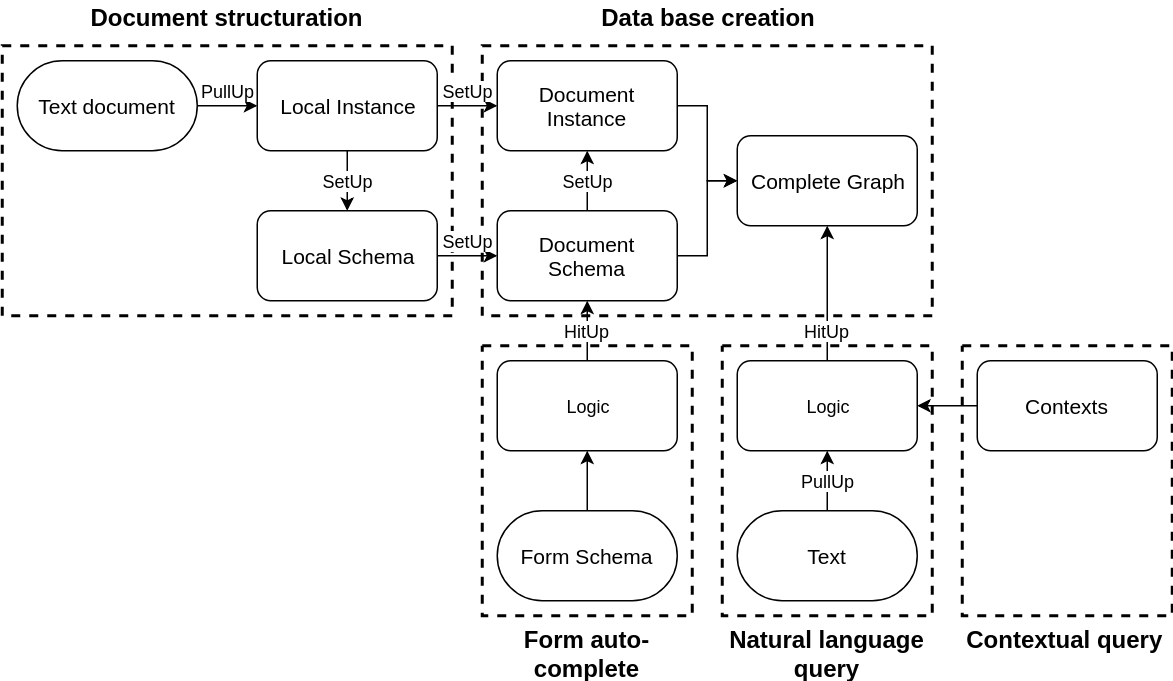
\includegraphics[width=\linewidth]{these/images/global_project.png}
%     \caption{Schéma du projet}
%     \label{fig:sch_projet}
% \end{figure}

% \paragraph{\gls{pullup}} est la partie s'occupant de l'extraction d'information.
% Elle a pour objectif d'extraire les connaissances contenues dans un texte formulé en langage naturel sous forme de faits logique pouvant être utilisés pour construire notre base de données par la suite.

% \paragraph{\gls{setup}} est un ensemble de travaux visant à construire dynamiquement une base de données cohérente par l'intermédiaire de grammaire de graphe \cite{chabin_using_2019}.
% Ces travaux sont réalisés conjointement avec l'équipe SDS du \gls{lifo}.
% Ils devraient permettre de s'assurer que la base reste cohérente sachant que l'on ne connaît pas la structure des données en entrée (car elles sont extraites depuis différents documents) et qu'on ne connaît pas le schéma de notre base (le schéma est propre aux documents présents dans la \gls{ged} et donc propre à chaque client).
% Bien que le processus puisse être réalisé manuellement, cette partie du projet vise donc à automatiser la construction de la base spécifique permettant de formuler des requêtes plus adaptées aux données qu'elle contient.

% \paragraph{\gls{hitup}} est une extension du formalisme présenté par \cite{chabin_context-driven_2018}.
% Il vise à fournir un langage de requête permettant d'effectuer des requêtes statistiques tout en ajoutant, via des réécritures, un contexte à la requête.
% Ce dernier peut être composé de contraintes d'intégrité ou de règles d'inférence utilisées pour spécifier la requête.

\section{Exemple}
\begin{quote}
    Un patient de 78 ans suivi pour cancer prostatique avec métastases ganglionnaires ayant déjà subi une résection endoscopique prostatique avec pulpectomie a été admis en urgence pour insuffisance rénale aiguë obstructive à 330 mmol/l de créatinine avec fièvre et urétérohydronéphrose bilatérale à l'échographie.
\end{quote}

\begin{align}
    CasClinique(\textit{c-2-3})  & exam(p_1, e_1, et_1, \textit{01-01-01}) \\
    hasPatient(\textit{c-2-3}, p1) & paramClinique(e_1, creatine, \textit{330mmol/L}) \\
    Patient(p_1, 78, H)  & reveal(e_1, \textit{insuffisance rénale}) \\
    hasPatho(p_1, cancer)  & exam(p_1, e_2, et_2, \textit{01-01-01}) \\
    concernsAnat(cancer, prostate) & paramClinique(e_2, temperature, t_1) \\
    Anatomy(prostate)  & reveal(e_2, fievre)  & exam(p_1, e_3, \textit{echographie}, \textit{01-01-01}) \\
    leadTo(cancer, \textit{métastases ganglionnaires})  & paramClinique(e_3, param_1, res_1) \\
    getTreatment(\textit{résection endoscopique}, prostate) & reveal(e_3, \textit{urétérohydronéphrose bilatérale}) \\
    forPatho(\textit{résection endoscopique}, cancer)
\end{align}

\begin{figure}
    \small
    \centering
    \begin{adjustbox}{varwidth=\linewidth,max height=\textheight}
        \begin{tikzpicture}[shorten >=2pt,thick,-Latex,node distance=3cm and 5cm,on grid]
            \node[labeled node] (patient) {Patient \nodepart{two} name: \emph{$p_1$}\\sex: \emph{H}\\age: \emph{78}};
            \node[labeled node, below=of patient] (exam1) {Exam \nodepart{two} name: \emph{constantes}};
            \node[labeled node, below=of exam1] (param1) {ParamClinique \nodepart{two} name: \emph{créatinine}\\value: \emph{330 mmol/l}};
            \node[labeled node, below=of param1] (sosy1) {SOSY \nodepart{two} name: \emph{insuffisance}\\~~~~~~~~~~\emph{rénale}};
            \node[labeled node, right=of exam1] (exam2) {Exam \nodepart{two} name: \emph{échographie}};
            \node[labeled node, below=of exam2] (param2) {ParamClinique \nodepart{two} name: \emph{unknown}\\ value: \emph{unknown}};
            \node[labeled node, below=of param2] (sosy2) {SOSY \nodepart{two} name: \emph{urétérohydronéphrose}\\~~~~~~~~~~\emph{bilatérale}};
            \node[labeled node, left=of param1] (param3) {ParamClinique \nodepart{two} name: \emph{temperature}\\ value: \emph{unknown}};
            \node[labeled node, below=of param3] (sosy3) {SOSY \nodepart{two} name: \emph{fièvre}};
            \node[labeled node, above=of param3] (cas) {CasClinique \nodepart{two} doc: \emph{c-2-3}};
            \node[labeled node, above=of cas] (testicule) {Anatomie \nodepart{two} name: \emph{testicule}};
            \node[labeled node, above=of patient] (traitement) {Traitement};
            \node[labeled node, above=of traitement] (traitmentType) {TraitmentType \nodepart{two} name: \emph{résection}\\~~~~~~~~~~\emph{endoscopique}};
            \node[labeled node, above=of testicule] (traitement2) {Traitement};
            \node[labeled node, above=of traitement2] (traitmentType2) {TraitmentType \nodepart{two} name: \emph{pulpectomie}};
            \node[labeled node, above=of exam2] (metastase) {Symptom \nodepart{two} name: \emph{métastases}\\~~~~~~~~~~\emph{ganglionnaires}};
            \node[labeled node, above=of metastase] (cancer) {Pathologie \nodepart{two} name: \emph{cancer}};
            \node[labeled node, above=of cancer] (prostate) {Anatomie \nodepart{two} name: \emph{prostate}};

            \path
            (cas) edge node[labeled edge, anchor=center] {hasPatient} (patient)
            (patient) edge node[labeled edge, anchor=center] {hasPatho} (cancer)
            (patient) edge node[labeled edge, anchor=center] {getTreatment} (traitement)
            (cancer) edge node[labeled edge, anchor=center] {concernsAnat} (prostate)
            (patient) edge node[labeled edge, anchor=center] {getTreatment} (traitement2)
            (cancer) edge node[labeled edge, anchor=center] {leadTo} (metastase)
            (traitement) edge node[labeled edge, anchor=center] {forPatho} (cancer)
            (traitement) edge node[labeled edge, anchor=center] {concernsAnat} (prostate)
            (traitement) edge node[labeled edge, anchor=center] {hasType} (traitmentType)
            (traitement2) edge node[labeled edge, anchor=center] {concernsAnat} (testicule)
            (traitement2) edge node[labeled edge, anchor=center] {hasType} (traitmentType2)
            (patient) edge node[labeled edge, anchor=center] {passExam} (exam1)
            (exam1) edge node[labeled edge, anchor=center] {reveal} (param1)
            (param1) edge node[labeled edge, anchor=center] {show} (sosy1)
            (patient) edge node[labeled edge, anchor=center] {passExam} (exam2)
            (exam2) edge node[labeled edge, anchor=center] {reveal} (param2)
            (param2) edge node[labeled edge, anchor=center] {show} (sosy2)
            (exam1) edge node[labeled edge, anchor=center] {reveal} (param3)
            (param3) edge node[labeled edge, anchor=center] {show} (sosy3)
            ;
        \end{tikzpicture}
    \end{adjustbox}
    \caption{Instance sous forme de graphe}
    \label{fig:runex:graph}
\end{figure}


\section{Organisation du manuscrit}

\section{Publications}
